\chapter{Introduction to Binary Classification}

The problem of data classification is very important in the modern world. The classification aims to find a relation between a set of objects and target variables based on some objects' properties. The properties of the objects are usually called features, and the target variables are usually called labels. Many real-world problems can be formulated as classification tasks:
\begin{itemize}
  \item \textbf{Medical Diagnonsis:} In medicine, the classification is often used to improve disease diagnosis. In such a case, the features are medical records such as the patient's blood tests, temperature, or roentgen images. The target variable is if the patient has some disease. For example, classification can be used to process mammogram images and detect cancer~\cite{viale2012current, levy2016breast}.
  \item \textbf{Internet Secutiry:} These days, the internet is a crucial part of our lives. With the increasing usage of the internet, the number of attacks increases as well. An essential part of the defense is intrusion detection systems~\cite{grill2016learning, scarfone2007guide} that search for malicious activities (network attacks) in network traffic. Classification can be used to improve such systems as shown in~\cite{giacinto2002intrusion, shanbhag2009accurate}.
  \item \textbf{Marketing:} In marketing, the task can be to classify customers based on their buying interests. Such information can be used to build a personalized recommendation system for customers and therefore increase income~\cite{kaefer2005neural, zhang2007building}.
\end{itemize}
Besides these three examples, applications of classification can be found in almost every academic or even industrial field. Furthermore, a vast number of algorithms try to solve classifications problems. Typically these algorithms consist of three phases:
\begin{itemize}
  \item \textbf{Training:} The classification problems usually fall into the category of supervised learning. It means that we assume the prior knowledge of the target classes in the training phase. The training data typically consists of pairs (sample, label) and can be described as follows
  \begin{equation*}\label{eq: training set}
    \mathcal{D}_{\mathrm{train}} = \Brac[c]{(\bm{x}_i, y_i)}_{i=1}^{n},
  \end{equation*}
  where the sample~$\bm{x}_i \in \R^d$ is a~$d$-dimensional vector of features that describes the object of interes and the label~$y_i \in \{1, 2, \ldots, k\}$ represents target class. Moreover~$n \in \N$ is a number of training samples and~$k \in \N$ is a number of target classes. In this phase, the algorithm uses the training data to learn a model, i.e., set model parameters according to some predefined criterion, to describe the training data as best as possible.
  \item \textbf{Validation:} All algorithms usually have some hyperparameters that can be changed to improve the resulting model. The validation phase is used to select the best hyperparameter settings that lead to the most performant and robust model.
  \item \textbf{Testing:} In the testing phase, the model is used to assign labels~$\hat{y}_i \in \{1, 2, \ldots, k\}$ to the data from the testing set, which is not known during the training phase.
\end{itemize}
The previous definition of the training set is general for any classification problem with multiple classes. However, we focus on the special subclass of classification problems called binary classification in this work. The binary classification is a special case of classification in which the number of classes is~$k=2.$ These two classes are usually referred to as negative and positive classes. Moreover, the positive class is usually the one we are more interested. Returning to example with cancer, the positive class would represent that the patient has cancer while the negative that the patient is healthy.

\begin{notation}[Dataset]\label{not: dataset}
  In this work, we use label~$0$ to encode the negative class and label~$1$ to encode the positive class. Moreover, by a dataset of size~$n \in \N$ we mean a set of pairs in the following form
  \begin{equation*}
    \mathcal{D} = \Brac[c]{(\bm{x}_i, y_i)}_{i=1}^{n},
  \end{equation*}
  where~$\bm{x}_i \in \R^d$ represents samples,~$d \in \N$ its dimension and~$y_i \in \{0, 1\}$ corresponding labels. To simplify future notation, we denote a set of all indices of dataset~$\mathcal{D}$ as~$\I = \Ineg \cup \Ipos,$ where
  \begin{equation*}
    \begin{aligned}
      \Ineg & = \Set{i}{i \in \{1, 2, \ldots, n\} \; \land \; y_i = 0}, \\
      \Ipos & = \Set{i}{i \in \{1, 2, \ldots, n\} \; \land \; y_i = 1}.
    \end{aligned}
  \end{equation*}
  We also denote the number of negative samples in~$\mathcal{D}$ as~$\nneg = \Brac[v]{\Ineg}$ and the number of positive samples in~$\mathcal{D}$ as~$\npos = \Brac[v]{\Ipos},$ i.e. total number of samples is~$n = \nneg + \npos.$ 
\end{notation}

The goal of any classification problem is to classify given samples with the highest possible accuracy or, in other words, with the lowest possible error. In the case of binary classification, there are two types of error: positive sample is classified as negative and vice versa. Formally, using the Notation~\ref{not: dataset}, the minimization of these two types of errors can be written as follows
\begin{mini}{\bm{w}, t}{
    \lambda_1 \sum_{i \in \Ineg} \Iverson{s_i \geq t} + \lambda_2 \sum_{i \in \Ipos} \Iverson{s_i < t}
  }{\label{eq: Binary classification}}{}
  \addConstraint{s_i}{= f(\bm{x}_i; \bm{w}), \quad}{i \in \I,}
\end{mini}
where~$\lambda_1, \lambda_2 \in \R,$ the function~$f \colon \R^d \to \R$ is called model and~$\Iverson{\cdot{}}$ is Iverson function that is used to counts misclassified samples and is defined as
\begin{equation}\label{eq: iverson}
  \Iverson{x} = \begin{cases}
    0 & \quad \text{if } x \text{ is false}, \\
    1 & \quad \text{if } x \text{ is true}.
  \end{cases}
\end{equation}
Moreover, the vector~$\bm{w} \in \R^d$ represents trainable parameters (weights) of the model~$f$ and~$t \in R$ represents a decision threshold. The parameters~$\bm{w}$ are determined from training data during the training phase of the algorithm. Although the decision threshold~$t$ can also be determined from the training data, in many cases, it is fixed. For example, many algorithms assume that the classification score~$s_i = f(\bm{x}_i; \bm{w})$ given by the model~$f$ represents the probability that the sample~$\bm{x}_i$ belongs to the positive class. Therefore, the decision threshold is set to~$t = 0.5,$ and the sample is classified as positive if its classification score is larger than this threshold. In Notation~\ref{not: classifier}, we summarize the notation that is used in the rest of the work.

\pagebreak

\begin{notation}[Classifier]\label{not: classifier}
  By classifier, we always mean pair of model~$f$ and corresponding decision threshold~$t$. By model, we mean a function $f \colon \R^d \to \R$ which maps samples~$\bm{x}$ to its classification scores~$s$, i.e. for all~$i \in \I$ the classification score is defined as
  \begin{equation*}
    s_i = f(\bm{x}_i; \; \bm{w}),
  \end{equation*}
  where~$\bm{w}$ represents trainable parameters (weights) of the model. Predictions are defined for all~$i \in \I$ in the following way
  \begin{equation*}
    \hat{y}_i = \begin{cases}
      1 & \quad \text{if } s_i \geq t, \\
      0 & \quad \text{otherwise.}
    \end{cases}
  \end{equation*}
\end{notation}

\section{Performance Evaluation}

In the previous section, we defined general binary classification problem~\ref{eq: Binary classification}. However, we did not discuss how to measure the performance of the resulting classifier. In this section, we introduce basic performance metrics  that are used to measure the performance of binary classifiers.

\subsection{Confusion Matrix}

Based on the prediction~$\hat{y}_i$ and an actual label~$y_i$ of the sample~$\bm{x}_i,$ each sample can be assigned to one of the four following categories:
\begin{itemize}
  \item \textbf{True negative:} sample~$\bm{x}_i$ is negative and is classified as negative, i.e.~$y_i = 0 \; \land \; \hat{y}_i = 0.$
  \item \textbf{False positive:} sample~$\bm{x}_i$ is negative and is classified as positive, i.e.~$y_i = 0 \; \land \; \hat{y}_i = 1.$
  \item \textbf{False negative:} sample~$\bm{x}_i$ is positive and is classified as negative, i.e.~$y_i = 1 \; \land \; \hat{y}_i = 0.$
  \item \textbf{True positive:} sample~$\bm{x}_i$ is positive and is classified as positive, i.e.~$y_i = 1 \; \land \; \hat{y}_i = 1.$
\end{itemize}
Using these four categories, we can construct a so-called confusion matrix (sometimes also called contingency table)~\cite{fawcett2006introduction} that represents the results of predictions for all samples from the given dataset~$\mathcal{D}$. An illustration of the confusion matrix is shown in Figure~\ref{fig: confusion matrix}. If we denote the vector of all classification scores given by model~$f$ as~$\bm{s} \in \R^n,$ we can compute all fields of the confusion matrix as follows
\begin{equation}\label{eq: confusion counts}
  \begin{aligned}
    \tp(\bm{s}, t) & = \sum_{i \in \Ipos}\Iverson{s_i \geq t}, & \quad
    \fn(\bm{s}, t) & = \sum_{i \in \Ipos}\Iverson{s_i < t}, \\
    \tn(\bm{s}, t) & = \sum_{i \in \Ineg}\Iverson{s_i < t}, & \quad
    \fp(\bm{s}, t) & = \sum_{i \in \Ineg}\Iverson{s_i \geq t}.
  \end{aligned}
\end{equation}
In the following text, we sometimes use simplified notation~$\tp = \tp(\bm{s}, t)$ (and similar notation for other counts) for example to define classification metrics. In such cases, the vector of classification scores and decision threshold is fixed and is known from the context. Using the simplified notation, we can define true-positive, false-positive, true-negative, and false-negative rates as follows
\begin{equation}\label{eq: confusion rates}
  \begin{aligned}
    \tpr & = \frac{\tp}{\npos}, & \quad
    \fnr & = \frac{\fn}{\npos}, & \quad
    \tnr & = \frac{\tn}{\nneg}, & \quad
    \fpr & = \frac{\fp}{\nneg}.
  \end{aligned}
\end{equation}
Figure~\ref{fig: scores and rates} shows the relation between classification rates and the decision threshold. The blue and red curves represent the theoretical distribution of the scores of negative and positive samples, respectively. The position of the decision threshold determines the values of the classification rates. The higher the decision threshold, the lower the false-positive rate, but at the same time, the higher the false-negative rate. Similarly, the lower the decision threshold, the higher the false-positive rate and the lower the false-negative rate. Ideally, classification without errors is the goal, but it is not usually possible. If we look at the general definition of the binary classification problem~\eqref{eq: Binary classification}, the objective function is just the weighted sum of false-positive and false-negative samples. Therefore, we can use the notation~\eqref{eq: confusion rates} and rewrite the problem~\eqref{eq: Binary classification} to the following form
\begin{mini}{\bm{w}, t}{
    \lambda_1 \cdot \fp(\bm{s}, t) + \lambda_2 \cdot \fn(\bm{s}, t)
  }{\label{eq: Binary classification counts}}{}
  \addConstraint{s_i}{= f(\bm{x}_i; \bm{w}), \quad}{i \in \I.}
\end{mini}
The parameters~$\lambda_1, \; \lambda_2 \in \R$ are used to specify which error is more serious for the particular classification task.

\begin{figure}
  \centering
  \begin{NiceTabular}{cccccc}[cell-space-limits = 7pt]
    && \Block[draw=black, line-width=2pt, rounded-corners]{1-2}{
      \textbf{Predicted label}
    } \\
    && $\hat{y} = 0$
    &  $\hat{y} = 1$
    && \Block{1-1}{\textbf{Row total:}} \\
    \Block[draw=black, line-width=2pt, rounded-corners]{2-1}{
      \rotate \textbf{Actual} \\ \textbf{label}
    }
    & $y = 0$
    & \Block[draw=mygreen, fill=mygreen!50, rounded-corners]{1-1}{
      true \\ negatives \\ (\textbf{tn})
    }
    & \Block[draw=myred, fill=myred!50, rounded-corners]{1-1}{
      false \\ positives \\ (\textbf{fp})
    }
    & $\rightarrow$
    & \Block[draw=black, rounded-corners]{1-1}{all \\ negatives \\ ($\nneg$)} \\
    & $y = 1$
    & \Block[draw=myred, fill=myred!50, rounded-corners]{1-1}{
      false \\ negatives \\ (\textbf{fn})
    }
    & \Block[draw=mygreen, fill=mygreen!50, rounded-corners]{1-1}{
      true \\ positives \\ (\textbf{tp})
    }
    & $\rightarrow$
    & \Block[draw=black, rounded-corners]{1-1}{all \\ positives \\ ($\npos$)} \\
    && $\downarrow$
    &  $\downarrow$ \\
    \Block{1-2}{\textbf{Column} \\ \textbf{total:}}
    && \Block[draw=black, rounded-corners]{1-1}{all predicted \\ negatives}
    & \Block[draw=black, rounded-corners]{1-1}{all predicted \\ positives}
  \end{NiceTabular}
  \caption{Representation of the confusion matrix for the binary classification problem, where the negative class has label~$0$ and the positive class has label~$1.$ The true (target) label is denoted as~$y$ and predicted label is denoted as~$\hat{y}.$}
  \label{fig: confusion matrix}
\end{figure}

\begin{figure}
  \centering
  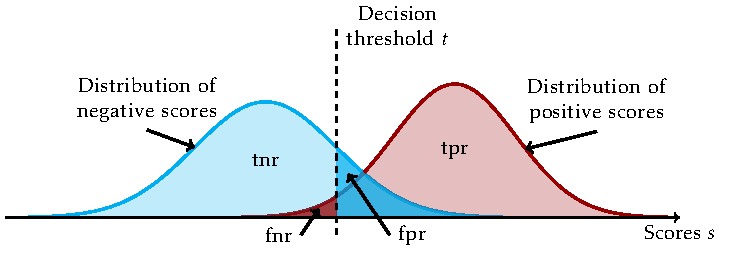
\includegraphics{images/confusion_rates.pdf}
  \caption{The relation between classification scores and  rates. The blue curve represents the theoretical distribution of the scores of negative samples, and the red curve the theoretical distribution of the scores of positive samples. Filled areas with light blue or light red represent true-negative and true-positive rates. Similarly, the filled areas with dark blue or dark red represent false-positive and false-negative rates.}
  \label{fig: scores and rates}
\end{figure}

The confusion matrix is not the only way to measure the performance of binary classifiers. For example, there are many different classification matrices, and many of them are derived directly from the confusion matrix~\cite{fawcett2006introduction, metz1978basic, brodersen2010balanced, hossin2015review}. As an example, we can mention accuracy and balanced accuracy defined as follows
\begin{align*}
  \accuracy & = \frac{\tp + \tn}{n} &
  \baccuracy & = \frac{\tpr + \tnr}{2}
\end{align*}
In the end of this chapter, we provide Table~\ref{tab: classification metrics} that summarizes all classification metrics used in this work. Moreover, in the following section, we introduce a different approach for the performance evaluation of binary classifiers.

\subsection{ROC Analysis}

In the previous section, we defined general binary clasification problem~\eqref{eq: Binary classification counts} that minimizes weighted sum of false-positive and false-negative counts. Therefore, we always have to find some trade-off between the false-positive and false-negative counts and select the best hyperparameters~$\lambda_1,$~$\lambda_1,$ for given tasks. There is no universal truth, which error is worse. For example, we may want to detect cancer from some medical data. In such a case, it is probably better to classify a healthy patient as sick than the other way around. On the other hand, in computer security, we do not want an antivirus program that makes a lot of false-positive alerts since it will be disruptive for the user. One way how to visualize the trade-off between false-positive and false-negative errors is using Receiver Operating Characteristic (ROC) space~\cite{egan1975signal, fawcett2006introduction}.

ROC space is a two-dimensional space with x-axis equal to false-positive rate and the y-axis to true-positive rate. The left-hand side of Figure~\ref{fig: roc space} shows ROC space with 5 highlighted points. Each point in ROC space represents one fixed classifier, i.e., one pair of model~$f$ and decision threshold~$t.$ There are several important points in ROC space. The point~$(0, 0)$ represents classifier that classifies all samples as negative, while the point~$(1, 1)$ represents classifier that classifies all samples as positive. Both these classifiers are useless. On the other hand, the point~$(0, 1)$ represents perfect classifier. Generally, we can say, that one classifier is better than another, if its representation in ROC space is to the northwest of the second one. In such a case, the classifier has higher true-positive rate and lower false-positive rate than the second one. For example, in Figure~\ref{fig: roc space}, classifier \textbf{B} is bettert than classifier \textbf{C}. On the other hand, it is possible to say which classifier is better if one has higher true-positive rate and the other has lower false-positive rate. We can see this situation for classifier \textbf{B} and \textbf{A}. In such a case, the preference depends on the given problem as disscused in the beggining of this section. 

Another important part of the ROC space is diagonal line highlighted in red in Figure~\ref{fig: roc space}. Any classifier that appears on this diagonal provides same performance as random classifier. For example, classifier \textbf{C} is represented in ROC space by point~$(0.7, 0.7).$ It means, that this classifier randomly classify 70\% of samples as positive. That means, that any classifier that apperas in ROC space in the lower roght triangle is worse than a random classifier. Therefore, there are usually no classifiers in this area. In fact, any classifier from the lower right triangle can be easily improved. If we negate the decision of such classifier for every sample, we get classifier in the upper left triangle. Such a situation is in Figure~\ref{fig: roc space} for classifier \textbf{E} and \textbf{B}. Since we negate every decision of classifier \textbf{E}, all true-positive samples became false-negative and vice versa. Since classifier \textbf{E} has false-negative rate 0.8, we can deduce that negated classifier will have true-positive rate 0.8. Similarly, since classifier \textbf{E} has true-negative rate 0.4, its negated version will have false-positive rate 0.4. Therefore the negated version of classifier \textbf{E} is represented in ROC space by point~$(0.4, 0.8),$ which is classifier \textbf{B}.

\begin{figure}
  \centering
  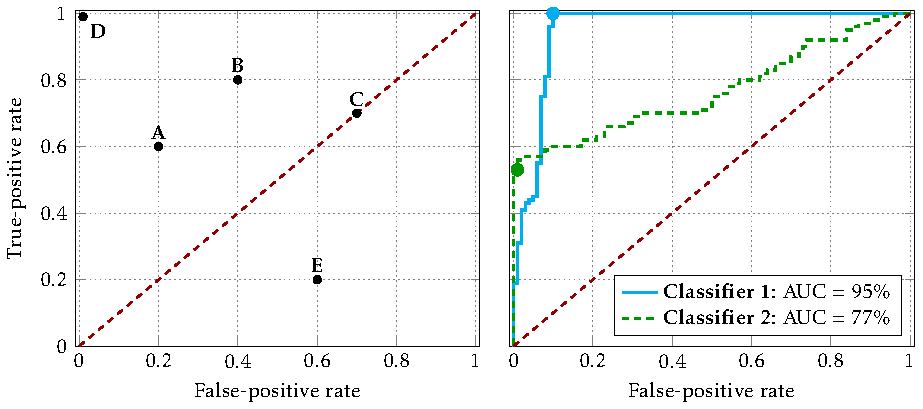
\includegraphics{images/roc_space.pdf}
  \caption{A basic representation of the ROC space with fiv different classifiers. (\textbf{left}) A comparison of ROC curves of two different classifiers. (\textbf{right})}
  \label{fig: roc space}
\end{figure}

Many classifier produce directly decision that samples are positive or negative. As an example, we can mention decision trees. Such classifiers are always represented as a single point in ROC space. Moreover, classifier that produce decision directly do not fit into our description from Notation~\ref{not: classifier}, since they not provide any classification scores. In this text, we always assume that classifier consists of the model~$f$ that for each sample produces a classification score, and the decision threshold~$t.$ Many standard classifiers such as neural networks or logistic regression fall into this settings. Even though the decision threshold is determined during the training process, it is possible to change it and obtain different predictions. This possibility is very often used to produce so called ROC curves~\cite{fawcett2006introduction}. ROC curves represents how model~$f$ behaves for different thresholds~$t$ varying from~$-\infty$ to~$+\infty.$ Right-hand side of Figure~\ref{fig: roc space} provides example of two ROC curves for two different classifiers. The first classifier~$(f_1, t_1)$ provides accuracy~95\% and is represented by orange dot, while its ROC curve is represented by orange line. The second classifier~$(f_2, t_2)$ represented by green dot provides accuracy~76\% and its ROC curve is represented by green line. A common method how to compare two classifiers using ROC curves is to compare corresponding areas under the ROC curve (AUC)~\cite{bradley1997use, hanley1982meaning}. This is a simple way how to reduce the ROC curve to on number, and for standard binary classification, the larger the area under the ROC curve is, the better. In Figure~\ref{fig: roc space} we can see that the orange classifier has AUC 95.3\% while the green one only 76.8\%. Therefore, for most classification problems, the orange classifier is better. 

Since both fale-positive and true-positive rates are non-increasing functions of threshold~$t,$ we can efficently compute the ROC curve from sorted classification score~$\bm{s}$ given by the model~$f.$ In Algorithm~\ref{alg: roc curve} we summarize and efficient algorithm for generating ROC curve. This algorithm gives us an interesting insight to ROC curves: ROC curves represent the ability of the model to rank the positive samples higher than the negative samples~\cite{fawcett2006introduction}. Moreover, AUC of a classifier is equivalent to the probability, that the classifier will rank randomly chosen positive sample higher than randomly chosen negative sample~\cite{fawcett2006introduction}. By comparing classifier from the right-hand side of Figure~\ref{fig: roc space}, we can deduce, that classifier 1 is generally better at false-positive rate larger than~$0.01$ while the second one otherwise. Therefore, even if the green classifier seems worse than the orange one, there is a specific region of ROC space in which is better. In the next section, we discuss special classification problems which focus on the performance only at low false-positive rates.

\begin{algorithm}
  \centering
  \begin{algorithmic}[1]
    \Require Sorted classification scores~$\bm{s}_{[\cdot]}$ in decreasing order~$s_{[1]} \geq \dots \geq s_{[n]}$
    \State Set $\tp \gets 0,$ $\fp \gets 0,$ $s_{\text{prev}} = +\infty,$ and an empty set~$ROC = \{~\}$ of points in ROC space
    \For{$l \in \{1, \ldots, \nall\}$}
      \If{$s_{[i]} \neq s_{\text{prev}}$} 
        \State push~$(\nicefrac{\fp}{\nneg}, \nicefrac{\tp}{\npos})$ into~$ROC$
      \EndIf
      \If{$y_{[i]} = 1$}
        \State $\tp \gets \tp + 1$
      \Else
        \State $\fp \gets \fp + 1$
      \EndIf
    \EndFor
    \State push~$(\nicefrac{\fp}{\nneg}, \nicefrac{\tp}{\npos}) = (1, 1)$ into~$ROC$
  \end{algorithmic}
  \caption{Efficient algorithm~\cite{fawcett2006introduction} for generating ROC curve from sorted classification scores.}
  \label{alg: roc curve}
\end{algorithm}

\section{Classification at the Top}\label{sec: related problems}

The aim of classical binary classification is to separate positive and negative samples with the highest possible accuracy. However, in many applications, it is desirable to separate only a certain number of samples. In such a case, the goal is not to maximize the performance on all samples but only the performance on the required samples with the highest relevance. The rest of the samples is irrelevant and therefore the performance on them is not important. Figure~\ref{fig: standard vs. aatp} shows the difference between the standard classifier (classifier 1) that maximizes the accuracy and the classifier that focuses only on the classification at the top (classifier 2). In this particular case, the classifier 2 tries to maximize the number of positive samples that are ranked higher than the worst negative sample, i.e. the negative sample with the highest score. Formally, classifier 2 maximizes the following metric
\begin{equation*}
  \postop(\bm{s}) = \frac{1}{\npos} \sum_{i \in \Ipos} \Iverson{s_i \geq \max_{j \in \Ineg}\{s_j\}}.
\end{equation*}
While classifier 1 has good total~$\accuracy$, its~$\postop$ metric is subpar because of the few negative outliers. On the other hand, classifier 2 has worse total~$\accuracy$, but its~$\postop$ metric is extremely good because more than half of the positive samples are ranked higher than the worst negative sample. While classifier 1 selected different thresholds for the~$\accuracy$ and~$\postop$ metrics, these thresholds coincide for classifier 2. In the rest of the chapter, we will present three main categories of problems that are closely related to the binary classification but do not focus on optimizing overall performance.

\begin{figure}
  \centering
  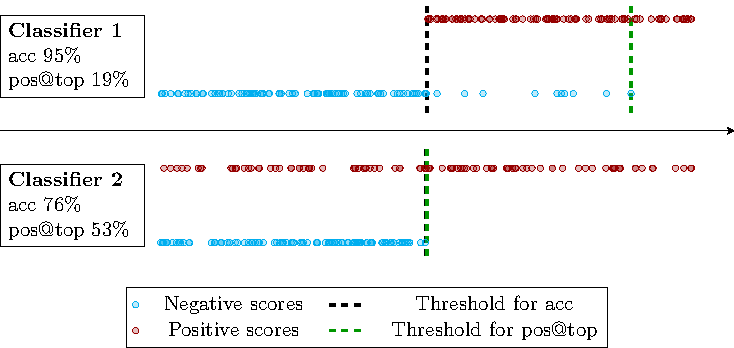
\includegraphics{images/standard_aatp_comparison.pdf}
  \caption{Difference between standard classifiers (\textbf{Classifier~1}) and classifiers maximizing~$\postop$ metric (\textbf{Classifier~2}). While the former has a good total~$\accuracy$, the latter has a~$\postop$ metric.}
  \label{fig: standard vs. aatp}
\end{figure}

\begin{figure}
  \centering
  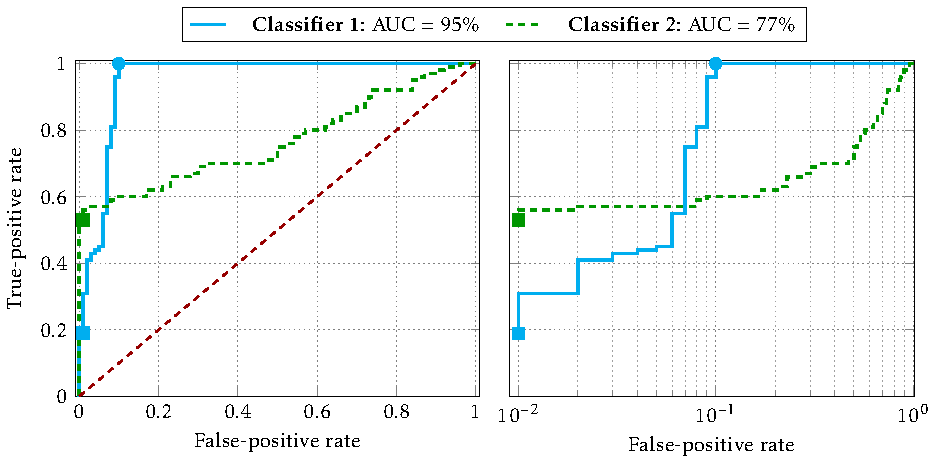
\includegraphics{images/roc_space_log.pdf}
  \caption{???}
  \label{fig: roc space log}
\end{figure}

\subsection{Ranking Problems}

\textbf{Ranking problems:} Ranking problems~\cite{freund2003efficient, agarwal2011infinite, rudin2009pnorm, li2014top} select the most relevant samples and rank them. To each sample, a numerical score is assigned, and the ranking is performed based on this score. Often, only scores above a threshold are considered. As an example, we can mention search engines such as Google, DucDucGo or Yahoo. In such a case, the goal is to provide most relevant results on the first two or three pages. The results on page 50 are usually of no interest to anyone, so it is important to move the most relevant results to the few first pages~\cite{cortes2003auc}.

The first category of problems that is tightly related to binary classification at the top, is the category of ranking problems. Ranking problems have become very important in many different fields
\begin{itemize}
  \item \textbf{Information retrieval systems:} The goal of the information retrieval systems is to rank documents according to relevance to a given query.
  \item \textbf{Recommendation  systems:} The goal is to rank and recommend products based on the user's previous behavior.
  \item 
\end{itemize}
All the examples above can be formulated as bipartite ranking problem~\cite{freund2003efficient, agarwal2005generalization, agarwal2011infinite}, where the goal is to rank the relevant (positive) samples higher than the non-relevant (negative) ones. 

Ranking problems~\cite{freund2003efficient, agarwal2011infinite, rudin2009pnorm, li2014top} select the most relevant samples and rank them. To each sample, a numerical score is assigned, and the ranking is performed based on this score. Often, only scores above a threshold are considered. As an example, we can mention search engines such as Google, DucDucGo or Yahoo. In such a case, the goal is to provide most relevant results on the first two or three pages. The results on page 50 are usually of no interest to anyone, so it is important to move the most relevant results to the few first pages~\cite{cortes2003auc}.

A prototypical example is the RankBoost~\cite{freund2003efficient} maximizing the area under the ROC curve, the Infinite Push~\cite{agarwal2011infinite} or the~$p$-norm push~\cite{rudin2009pnorm} which concentrate on the high-ranked negatives and push them down. Since all these papers include pairwise comparisons of all samples, they can be used only for small datasets. This was alleviated in~\cite{li2014top}, where the authors performed the limit~$p \to \infty$ in~$p$-norm push and obtained the linear complexity in the number of samples. Moreover, since the~$l_{\infty}$-norm is equal to the maximum, this method falls into our framework with the threshold equal to the largest score computed from negative samples.

Many methods, such as \emph{RankBoost}~\cite{freund2003efficient}, \emph{Infinite Push}~\cite{agarwal2011infinite} or \emph{$p$-norm push}~\cite{rudin2009pnorm} employ a pairwise comparison of samples, which makes them infeasible for larger datasets. This was alleviated in \TopPush~\cite{li2014top} where the authors considered the limit~$p \rightarrow \infty$. Since the~$l_{\infty}$ norm from \TopPush is equal to the maximum, the decision threshold from our framework equals to the maximum of scores of negative samples. This was generalized into \TopPushK~\cite{adam2021general} by considering the threshold to be the mean of~$K$ largest scores of negative samples.

\subsection{Accuracy at the Top}

\textbf{Accuracy at the Top:} Accuracy at the Top~\cite{boyd2012accuracy, grill2016learning} is similar to ranking problems. However, instead of ranking the most relevant samples, it only maximizes the number of positive samples (equivalently minimizes the misclassification)  above the top~$\tau$-quantile of scores. The Accuracy at the Top can be very useful for search engines or in applications where identified samples undergo expensive post-processing such as human evaluation. As an example, we can mention cyber security~\cite{grill2016learning}, where a low false-negative rate is crucial as a high number of false alarms would result in the software being uninstalled, or drug development, where potentially useful drugs need to be preselected and manually investigated.

Accuracy at the Top ($\tau$-quantile) was formally defined in~\cite{boyd2012accuracy} and maximizes the number of relevant samples in the top~$\tau$-fraction of ranked samples. When the threshold equals the top~$\tau$-quantile of all scores, this problem falls into our framework. The early approaches aim at solving approximations, for example,~\cite{joachims2005svm} optimizes a convex upper bound on the number of errors among the top samples. Due to the presence of exponentially many constraints, the method is computationally expensive.~\cite{boyd2012accuracy} presented an SVM-like formulation which fixes the index of the quantile and solves~$n$ problems. While this removes the necessity to handle the (difficult) quantile constraint, the algorithm is computationally infeasible for a large number of samples.~\cite{kar2015surrogate} derived upper approximations, their error bounds and solved these approximations.~\cite{grill2016learning} proposed the projected gradient descent method where after each gradient step, the quantile is recomputed.~\cite{eban2017scalable} suggested new formulations for various criteria and argued that they keep desired properties such as convexity.~\cite{tasche2018plug} showed that accuracy at the top is maximized by thresholding the posterior probability of the relevant class. The closest approach to our framework is~\cite{lapin2015top,lapin2018analysis}, where the authors considered multi-class classification problems, and their goal was to optimize the performance on the top few classes and~\cite{mackey2018constrained}, where the authors implicitly removed some variables and derived an efficient algorithm.

\AccatTop~\cite{boyd2012accuracy} focuses on maximizing the number of positive samples above the top~$\tau$-quantile of scores. There are many methods on how to solve accuracy at the top. In~\cite{boyd2012accuracy}, the authors assume that the top quantile is one of the samples, construct~$n$ unconstrained optimization problems with fixed thresholds, solve them and select the best solution. This method is computationally expensive. In~\cite{grill2016learning} the authors propose a fast projected gradient descent method. In our previous paper, we proposed a convex approximation of the accuracy at the top called \PatMat. This method is reasonably fast and guaranteed the existence of global optimum.

\subsection{Hypothesis Testing}

\textbf{Hypothesis testing} states a null and an alternative hypothesis. The Neyman-Pearson problem minimizes the Type II error (the null hypothesis is false but it fails to be rejected) while keeping the Type I error (the null hypothesis is true but is rejected) small. If the null hypothesis states that a sample has the positive label, then Type II error happens when a positive sample is below the threshold and thus minimizing the Type II error amounts to minimizing the positives below the threshold.

Hypothesis testing states a null and an alternative hypothesis. The Neyman-Pearson problem minimizes the Type II error (the null hypothesis is false but it fails to be rejected) while keeping the Type I error (the null hypothesis is true but is rejected) small. If the null hypothesis states that a sample has the positive label, then Type II error happens when a positive sample is below the threshold and thus minimizing the Type II error amounts to minimizing the positives below the threshold.

\subsection{related work deep}

There is a close connection between accuracy at the top and ranking problems~\cite{batmaz2019review,werner2019review}. This was, together with similarities to the Neyman-Pearson problem, showed in~\cite{adam2021general}. A special case of the ranking problems attempts to rank positive samples above negative samples. Several approaches, such as RankBoost~\cite{freund2003efficient}, Infinite Push~\cite{agarwal2011infinite} or~$p$-norm push~\cite{rudin2009pnorm} employ a positive-negative pairwise comparison of scores, which can handle only small datasets. TopPush~\cite{li2014top} converts the pairwise sum into a single sum and minimizes the false-negatives below a threshold given by the maximum score corresponding to negative samples. Thus, it converts ranking into accuracy at the top problems.

Two approaches for solving \eqref{eq:problem} exist. The first approach considers the threshold constraint as it is, while the second approach uses heuristics to approximate it. In the first approach, Acc@Top~\cite{boyd2012accuracy} argues that the threshold equals one of the scores. They fix the index of a sample and solve as many optimization problems as there are samples.~\cite{eban2017scalable,adam2021general,kumar2021implicit} write the threshold as a constraint and replace both the objective and the constraint via surrogates.~\cite{eban2017scalable} uses Lagrange multipliers to obtain a minimax problem,~\cite{mackey2018constrained} implicitly removes the threshold as an optimization variable and uses the chain rule to compute the gradient while~\cite{macha2020nonlinear} solves an SVM-like dual formulation with kernels.~\cite{grill2016learning} uses the same formulation but applies surrogates only to the objective and recomputes the threshold after each gradient step. \TFCO~\cite{cotter2019optimization} solves a general class of constrained problems via a minimax reformulation. In the second approach, SoDeep~\cite{engilberge2019sodeep} or SmoothI~\cite{thonet2021smoothi} use the fact that the threshold may be easily computed from sorted scores. They approximate the sorting operator by a network trained on artificial data. \APPerf~\cite{fathony2019ap} considers a general metric and hedges against the worst-case perturbation of scores. The authors argue that the problem is bilinear in scores and use duality arguments. However, the bilinearity is lost when optimizing with respect to the weights of the original network. 

\section{Summary}


\begin{table}
  \centering
  \begin{NiceTabular}{ccc}
    \CodeBefore
      \rowcolor{\headercol}{1}
      \rowcolors{3}{\rowcol}{}[restart]
    \Body
    \toprule
    \textbf{Name} & \textbf{Aliases} & \textbf{Formula} \\
    \midrule
    true negatives
      & correct rejection
      & $\tn$ \\
    false positives
      & Type I error, false alarm
      & $\fp = \nneg - \tn$ \\
    true positives
      & hity
      & $\tp$ \\
    false negatives
      & Type II error
      & $\fn = \npos - \tp$ \\
    \midrule
    true negative rate
      & specificity, selectivity
      & $\tnr = \frac{\tn}{\nneg}$ \\
    false positive rate
      & fall-out
      & $\fpr = \frac{\fp}{\nneg} = 1 - \tnr$ \\
    true positive rate
      & sensitivity, recall, hit rate
      & $\tpr = \frac{\tp}{\npos}$ \\
    false negative rate
      & miss rate
      & $\fnr = \frac{\fn}{\npos} = 1 - \tpr$ \\
    \midrule
    accuracy
      & ---
      & $\accuracy = \frac{\tp + \tn}{n}$ \\
    balanced accuracy
      & ---
      & $\baccuracy = \frac{\tpr + \tnr}{2}$ \\
    precision
      & positive predictive value
      & $\precision = \frac{\tp}{\tp + \fp}$ \\
    \bottomrule
  \end{NiceTabular}
  \caption{Summary of classification metrics derived from confusion matrix. The first column shows the name used in this work, while the second column shows alternative names that can be found in the literature. The last column shows the formula based on the confusion matrix.}
  \label{tab: classification metrics}
\end{table}